\documentclass[10pt,twocolumn,letterpaper]{article}

\usepackage{times}
\usepackage{graphicx}
\usepackage{float}
\usepackage[italian]{babel}
\usepackage{csvsimple}
\usepackage[shortlabels]{enumitem}
\usepackage{listings}
\usepackage{multirow}
\begin{document}


\title{Integral Image Generator\\
\large Parallel Programming for Machine Learning\\Project Work in Artificial Intelligence Programming}

\author{Sofia Galante\\
\small sofia.galante@stud.unifi.it\\
}
\date{}
\maketitle
\thispagestyle{empty}

\section{Introduzione}

Il progetto svolto è un generatore di immagini integrali.\\
In un’immagine integrale, data un’immagine di partenza, ogni pixel è ottenuto sommando se stesso con tutti i pixel precedenti (sia lungo l’asse x che lungo l’asse y).\\
Si sono creati diversi generatori di immagini integrali:
\begin{enumerate}
\item{\textit{un generatore sequenziale}: in questo caso si generano le immagini integrali con un algoritmo sequenziale;}
\item{\textit{due versioni di un generatore con CUDA}: in questo caso si utilizza la GPU per parallelizzare la creazione dell’immagine integrale;}
\item{\textit{tre versioni di un generatore con OpenMP}: in questo caso si compie una parallelizzazione a livello della CPU del codice tramite OpenMP.}
\end{enumerate}
Lo scopo del progetto è quello di osservare lo speedup ottenuto nelle due versioni parallele dell’algoritmo, osservando anche quale parallelizzazione (tra GPU e CPU) risulta più efficiente.\\
Tutti gli esperimenti sono stati svolti su un PC con sistema operativo Windows 10, una CPU Intel Core i5-11400 e una GPU RTX 3070Ti.\\
La versione sequenziale e quella parallelizzata a livello di GPU utilizzano Visual C++ come compilatore, in quanto CUDA è compatibile solo con questo.\\
Per quanto riguarda la versione con OpenMP, si è optato per l’utilizzo di MinGW, in quanto Visual C++ dava problemi nell’annidare i cicli di parallel for.


\section{Organizzazione del codice}
\begin{figure}[H]
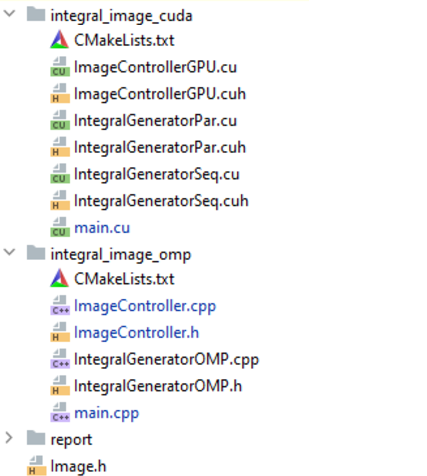
\includegraphics[width=0.7\linewidth]{code/org.png}
\caption{\small Organizzazione del codice}
\label{organizzazione}
\end{figure}
Il codice è stato suddiviso in due diversi progetti (si è utilizzato CLion come IDE): un progetto che utilizza Visual C++, e uno che utilizza MinGW. Inoltre un file .h è condiviso da entrambi i progetti.


\subsection{Il file condiviso: Image.h}

Il file condiviso da entrambi i progetti è il file \textbf{Image.h}, il quale contiene al suo interno la definizione di immagine, cioè una struct che ha come attributi una larghezza (\textit{width}), un’altezza (\textit{height}) e un puntatore di interi (\textit{pixels}) ad una locazione in memoria, la quale viene allocata dinamicamente durante l'esecuzione del programma.\\
Si noti che l'allocazione del puntatore di interi viene svolta con \textit{malloc()} se l’immagine è salvata nella CPU e con \textit{cudaMalloc()} se è invece salvata sulla GPU.\\
\\
Questo file contiene anche una variabile globale (\textit{SEED}), utilizzata come seed per la generazione di numeri casuali in entrambi i progetti, così da generare le stesse immagini.


\subsection{I file del progetto con compiler Visual C++}

Il primo progetto svolge i test di tipo sequenziale e quelli di tipo parallelo su GPU e li salva in appositi file csv.\\
I file presenti in questo progetto sono:

\begin{enumerate}
\item{\textbf{ImageController.cuh/cu}: i file che contengono la definizione e la dichiarazione di tutte le funzioni che si possono svolgere su un’Image. In particolare, si hanno una funzione per generare un’immagine casuale (\textit{generateImage()}), una funzione per copiare un’immagine (\textit{copyImage()}), funzioni per allocare/deallocare un’immagine dalla memoria (\textit{allocateImage(), freeHostImage(), freeDeviceImage()}) e funzioni per copiare un’immagine sulla CPU dalla GPU e viceversa (\textit{copyFromDeviceToHost() e copyFromHostToDevice()}.}
\item{\textbf{IntegralGeneratorSeq.cuh/cu}: i file che contengono la definizione e la dichiarazione della funzione necessaria a svolgere l’algoritmo sequenziale (\textit{generateIntegralCPUseq()});}
\item{\textbf{IntegralGeneratorPar.cuh/cu}: i file che contengono la definizione e la dichiarazione di due funzioni che implementano due diversi algoritmi paralleli con CUDA (\textit{generateIntegralGPUglobalMem() e generateIntegralGPUsharedMem()}) e le funzioni \textit{setup()} e \textit{finish()} utilizzate per allocare, copiare e deallocare tutte le immagini necessarie su CPU e GPU; come detto sopra, si sono scritte due diverse implementazioni dell’algoritmo di tipo parallelo e, di questo, ne parleremo nel dettaglio nella sezione dedicata (la 3);}
\item{\textbf{main.cu}: il file contenente tutte le funzioni relative ai test da svolgere e la funzione \textit{main()} del programma; si noti che quest'ultima riceve dall'esterno il nome del file con cui salvare i test svolti.}
\end{enumerate}


\subsection{I file del progetto con compiler MinGW}

Il secondo progetto si occupa di svolgere i test di tipo parallelo su CPU (con l’utilizzo di OpenMP) e di scrivere il risultato in relativi file csv.\\
I file presenti in questo progetto sono:
\begin{enumerate}
\item{\textbf{ImageController.h/cpp}: questi file contengono le funzioni riguardanti le immagini salvate su CPU presenti in ImageController.cuh del primo progetto.}
\item{\textbf{IntegralGeneratorOMP.h/cpp}: i file che contengono al loro interno la dichiarazione e la definizione di tre funzione che svolgono l’algoritmo parallelo con OpenMP (\textit{generateIntegralCPUompFirstLevel(), generateIntegralCPUompSecondLevel() e generateIntegralCPUompBothLevels()}).}
\item{\textbf{main.cpp}: il file contenente tutte le funzioni relative ai test da svolgere e la funzione \textit{main()} del programma; si noti che quest'ultima riceve dall'esterno il nome del file con cui salvare i test svolti.}

\end{enumerate}


\section{Parallelizzazione con CUDA}
In \textbf{IntegralGeneratorPar} si trovano due diverse implementazioni dello stesso algoritmo parallelo.\\
\\
La prima di queste (\textit{generateIntegralGPUglobalMem()}) è una parallelizzazione diretta della versione sequenziale dell’algoritmo: in questo caso ogni thread processa un singolo elemento dell’immagine e l’immagine originale e quella risultante si trovano entrambe nella memoria globale.\\
Questo tipo di algoritmo è penalizzato dai numerosi accessi alla \textbf{global memory} (uno ogni volta che si legge un elemento dell’immagine) che causano un aumento dell’effettivo tempo necessario.
\begin{figure}[H]
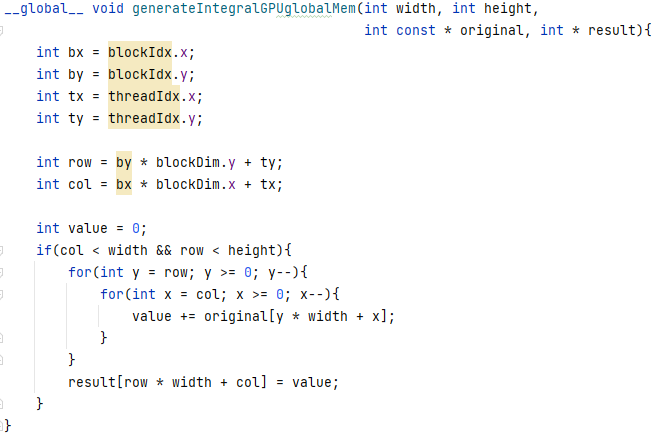
\includegraphics[width=1\linewidth]{code/cuda1.png} 
\caption{\small CUDA - Global Memory}
\label{cudacode1}
\end{figure}
La seconda versione dell’algoritmo (\textit{generateIntegralGPUsharedMem()}) utilizza la \textbf{shared memory} e la tecnica del \textbf{tiling} per risolvere il rallentamento dato dai continui accessi in global memory. La shared memory utilizzata viene allocata dinamicamente e dipende dalle dimensioni del blocco.\\
In questo algorimto, i thread di un blocco collaborano per caricare in shared memory gli elementi dell’immagine originale necessari per il calcolo. In particolare, l’algoritmo è stato diviso in fasi: ogni fase riguarda il caricamento di una quantità di elementi in shared memory pari alla grandezza di un block. Il numero di fasi di ogni block dipende dalla sua posizione nella grid: esso deve infatti caricare un numero di blocchi in memoria pari alla cardinalità dell'insieme di blocchi composto da sé stesso e dai blocchi che lo precedono (cioè che hanno indice x e/o y inferiore al suo).
\begin{figure}[H]
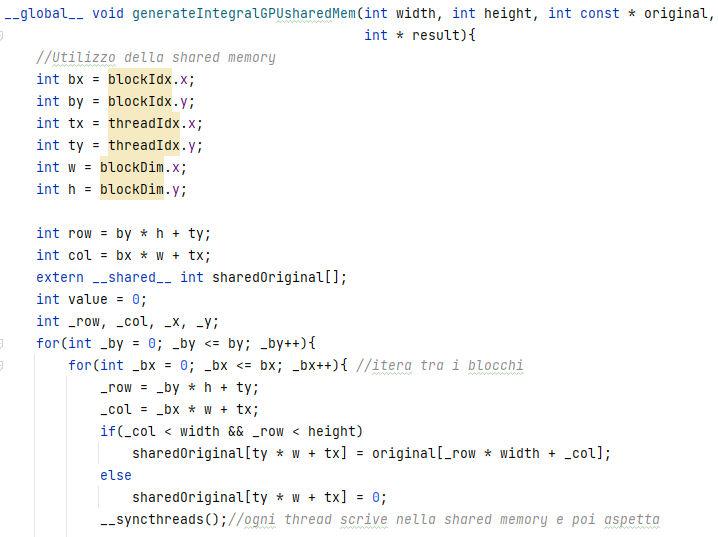
\includegraphics[width=1\linewidth]{code/cuda2_1.png} 
\caption{\small CUDA - Shared Memory (Prima parte)}
\label{cudacode2}
\end{figure}
Una volta caricati i blocchi in shared memory, i vari thread calcolano un valore parziale del risultato e, alla fine di tutte le fasi, ogni thread copia il valore calcolato nel pixel dell’immagine risultante.
\begin{figure}[H]
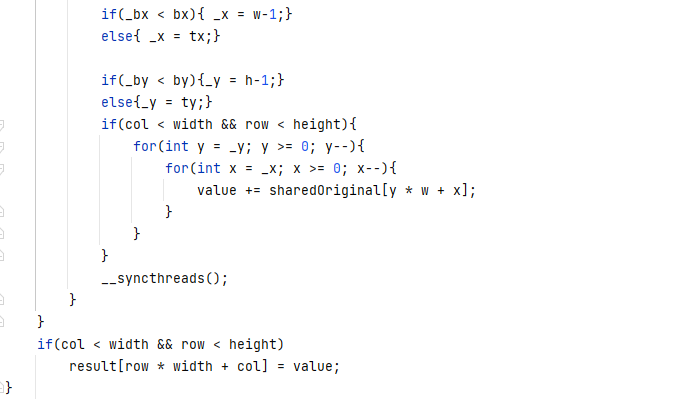
\includegraphics[width=1\linewidth]{code/cuda2_2.png} 
\caption{\small CUDA - Shared Memory (Seconda parte)}
\label{cudacode3}
\end{figure}
Si noti che, a differenza dell'algoritmo precedente, in questo sono presenti due chiamate alla funzione di sincronizzazione dei thread: questa funzione è necessaria in quanto, se non ci fosse, alcuni thread potrebbero (1) iniziare a calcolare il valore parziale del risultato prima che la shared memory sia stata tutta copiata e/o (2) iniziare a riscrivere la shared memory prima che un altro thread abbia finito il suo calcolo. Inserendo quelle due sincronizzazioni, questi fatti vengono evitati.\\
\\
Infine si vuole far notare che per osservare un effettivo miglioramento nell’utilizzo del secondo algoritmo rispetto al primo si è dovuta disattivare manualmente attraverso il CMake la cache di primo livello: il compilatore infatti salvava nella cache gli elementi da leggere, rendendo il primo algoritmo veloce quanto (se non, in alcuni casi, più) del secondo.


\section{Parallelizzazione con OpenMP}
La parallelizzazione dell’algoritmo svolta con l’utilizzo di OpenMP si trova in \textbf{IntegralGeneratorOMP}.\\
In questo caso, la parallelizzazione è stata effettuata con due diverse direttive \textit{omp parallel for}, annidate una dentro l'altra.\\
\\
La prima direttiva \textit{omp parallel for} (annidata a due livelli) parallelizza i due cicli for che danno le coordinate dell'elemento dell'immagine da calcolare.\\
Questa parallelizzazione è stata chiamata nel programma parallelizzazione al \textbf{primo livello}.\\
\\
La seconda direttiva \textit{omp parallel for} (anche questa annidata a due livelli) parallelizza invece il calcolo dell'elemento selezionato in precedenza. Visto che il calcolo di ogni pixel deriva da una somma di tutti i pixel precedenti, per sfruttare al meglio le risorse di OpenMP si è deciso di utilizzare una \textit{reduction}.\\
Questa parallelizzazione è stata chiamata nel programma parallelizzazione al \textbf{secondo}.\\
\\
Si noti che la scrittura nell'immagine risultante non è stata marcata come sezione critica in quanto ogni thread modifica un diverso elemento dell'immagine, non causando quindi alcuna race condition.\\
\begin{figure}[H]
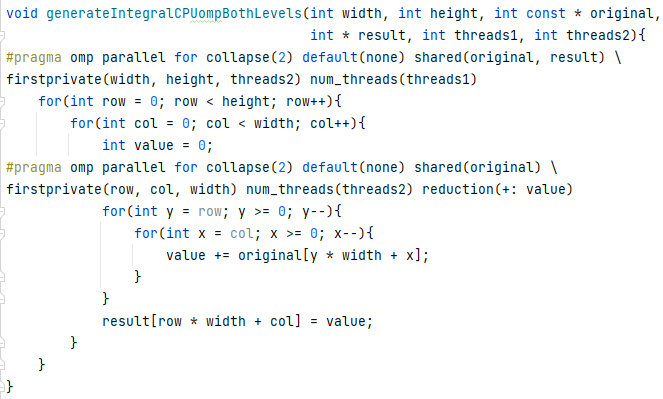
\includegraphics[width=1\linewidth]{code/omp3.png} 
\caption{\small OpenMP - parallelizzazione a entrambi i livelli}
\label{ompcode}
\end{figure}
Per osservare tutti i possibili risultati, si è deciso di creare tre diversi algoritmi di generazione dell'immagine integrale:
\begin{enumerate}
\item{\textit{generateIntegralCPUompFirstLevel()}, che contiene solo la parallelizzazione del primo livello;}
\item{\textit{generateIntegralCPUompSecondLevel()}, che contiene solo la parallelizzazione del secondo livello;}
\item{\textit{generateIntegralCPUompBothLevels()}, che contiene entrambe le parallelizzazioni (ed è la funzione riportata in figura).}
\end{enumerate}

\section{Esperimenti svolti}
Per osservare lo \textit{speedup} ottenuto dalla parallelizzazione del codice si sono compiuti diversi esperimenti.\\
In particolare si sono svolti tre diversi test, ognuno dei quali studia l'aumento del tempo di esecuzione al variare di alcuni parametri.\\
I test svolti sono:
\begin{enumerate}
\item{un test che osserva come il tempo di esecuzione per i due algoritmi su GPU si modifichi al variare della dimensione dei block e della grid e quale dei due algoritmi sia il migliore;}
\item{un test che confronta i diversi livelli di parallelizzazione dell'algoritmo di OpenMP, trovando il migliore e facendo poi un test su quest'ultimo per vedere come si comporta all'aumentare dei thread;}
\item{un test che confronta il tempo di esecuzione dell'algoritmo sequenziale, del miglior algoritmo CUDA e del miglior algoritmo OpenMP al variare della dimensione del labirinto.}
\end{enumerate}
Tutti gli esperimenti sono stati lanciati dal programma python \textbf{tests.py}. Ogni esperimento è stato svolto 10 volte. I risultati sono stati ottenuti facendo la media del tempo di esecuzione di ogni run (dopo aver eliminato i tempi massimi e minimi ottenuti). Tutti i risultati (sia quelli delle singole iterazioni dei test, sia quelli finali) sono salvati in appositi file csv. Per gli esperimenti si sono utilizzate delle immagini quadrate.\\
Il programma ha anche generato i grafici riportati in seguito.

\subsection{Variazione delle dimensioni dei block e della grid - CUDA}
Questo esperimento studia come si modificano i tempi di esecuzione dei due algoritmi CUDA al variare della dimensione della grid e dei block.\\
Si sono svolte due diverse versioni di questo esperimento.\\

\subsubsection{Studio dei casi limite}
Nella prima versione si sono scelte tre immagini di dimensione fissa (10x10, 100x100 e 1000x1000) e si sono osservati i casi limite per le dimensioni di block e grid, in particolare si sono studiati i seguenti casi:
\begin{enumerate}[-]
\item{\textbf{immagine divisa in righe}: in questo caso l'immagine è stata divisa in righe e ogni riga assegnata a un blocco;}
\item{\textbf{immagine divisa in colonne}: in questo caso l'immagine è stata divisa in colonne e ogni colonna è stata assegnata a un blocco;}
\item{\textbf{massimizzazione del numero di block nella grid}: in questo caso si sono usati più block possibili;}
\item{\textbf{massimizzazione del numero di thread per block}: in questo caso si sono usati più thread per block possibili.}
\end{enumerate}
I valori effettivi delle dimensioni di grid e block per le tre immagini possono essere visti nella tabella qui sotto:
\begin{table}[H]
\centering
\begin{tabular}{ |cc||c|c|c| } 
\hline
& & \multirow{2}{3em}{dim 10x10} & \multirow{2}{4em}{dim 100x100} & \multirow{2}{4em}{dim 1000x1000} \\
& & & & \\
\hline
\hline
\multirow{2}{3em}{righe} & grid & 1x10 & 1x100 & 1x1000 \\\cline{2-5} 
 & block & 10x1 & 100x1 & 1000x1 \\
\hline
\hline
\multirow{2}{3em}{colonne} & grid & 10x1 & 100x1 & 1000x1 \\\cline{2-5}
 & block & 1x10 & 1x100 & 1x1000 \\ 
\hline
\hline
\multirow{2}{3em}{max n° blocks} & grid & 10x10 & 100x100 & 255x255 \\\cline{2-5}
 & block & 1x1 & 1x1 & 4x4 \\
\hline
\hline
\multirow{2}{3em}{max n° threads} & grid & 1x1 & 4x4 & 32x32 \\\cline{2-5}
 & block & 10x10 & 32x32 & 32x32 \\ 
\hline
\end{tabular}
\caption{Tabella con dimensioni di griglia e blocco per ogni immagine}
\label{tab1}
\end{table}
Si noti che in alcuni casi nella massimizzazione del numero di block e nella massimizzazione del numero di thread i valori non corrispondono alla grandezza effettiva dell'immagine: questo accade in quanto, se si usassero la larghezza e l'altezza dell'immagine, si supererebbero i valori limite per numero di thread in un block (1024) e/o per numero di block in una grid (65535).\\
\\
I risultati ottenuti sono i seguenti:

\begin{table}[H]
\csvautotabular[separator=semicolon]{test/gridTest/size10/result.csv}
\caption{Immagine 10 x 10}
\end{table}
\begin{table}[H]
\csvautotabular[separator=semicolon]{test/gridTest/size100/result.csv}
\caption{Immagine 100 x 100}
\end{table}
\begin{table}[H]
\csvautotabular[separator=semicolon]{test/gridTest/size1000/result.csv}
\caption{Immagine 1000 x 1000}
\end{table}
Osservando le tre tabelle ottenute, si possono fare le seguenti considerazioni:
\begin{enumerate}
\item{L'algoritmo con memoria di tipo shared è più veloce di quello con memoria globale, tranne quanto la dimensione dei blocchi è troppo piccola (nei due casi in cui i blocchi hanno dimensioni 1 x 1, questo algoritmo è più lento); questo può essere spiegato facilmente dal fatto che, se il blocco è di dimensioni unitarie, allora la shared memory è inutile da utilizzare, in quanto si deve accedere ai valori copiati solo una volta. Si noti che basta che la dimensioni aumenti di poco (come nel caso 4 x 4) per far tornare vantaggioso l'utilizzo della shared memory.}
\item{In quasi tutti i casi, la divisione in righe comporta algoritmi più veloci della divisione in colonne; ciò è dato dal fatto che, nella divisione in righe, thread consecutivi devono accedere in posizioni consecutive della memoria (fanno degli accessi \textit{coalesced}) permettendo alle DRAM di rendere disponibili i dati con una burst (il tempo per accedere in memoria viene ridotto a quello di un singolo accesso). Nel caso della divisione per colonne, invece, questo non accade e i tempi si allungano.}
\item{Massimizzare la grandezza dei blocchi sembra essere molto più efficiente (all'aumentare dell'immagine) di massimizzare la grandezza della griglia.}
\end{enumerate}

\subsubsection{Studio di block di dimensioni multiple di 32}
Nella seconda versione del test ci siamo concentrati su dimensioni quadrate multiple di 32 per i block.\\
Questa scelta è stata dettata dal fatto che i thread all'interno di un block sono divisi a gruppi di 32 nei warp. Utilizzare una dimensione di block diversa da un multiplo di 32, quindi, comporterebbe comunque alla generazione di un numero di thread multipli di 32 per quel block, i quali resterebbero inattivi durante il processo.\\
Per osservare quale tra le tre dimensioni quadrate ammissibili multiple di 32 (8x8, 16x16 e 32x32) fosse la migliore per il nostro esperimento, si sono svolte più iterazioni dei due algoritmi CUDA (una per ognuna delle tre dimensioni) e si è osservato come i tempi di esecuzione variassero all'aumentare della dimensione dell'immagine (la quale parte da 10x10 e arriva fino a 500x500, aumentando il lato di 10 in 10).\\
\\
Il grafico totale ottenuto è il seguente:
\begin{figure}[H]
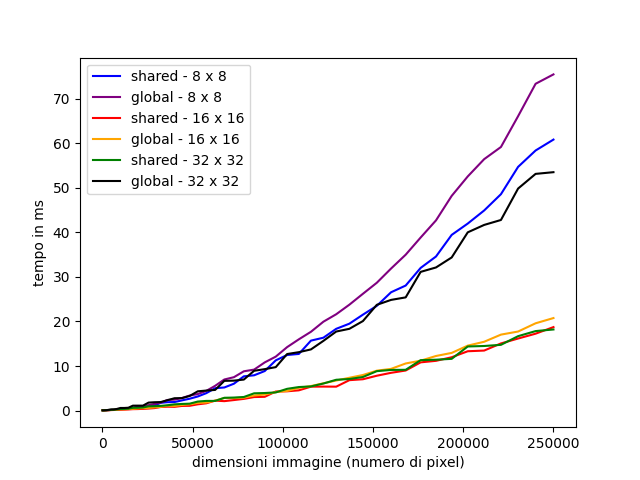
\includegraphics[width=0.9\linewidth]{test/gridTest/mul32/result.png} 
\caption{\small Tempo impiegato dall'esecuzione parallela al variare della dimensione dell'immagine.}
\label{t2_3}
\end{figure}
da cui si può osservare come gli algoritmi con shared memory siano superiori, a parità di grandezza dei block, a quelli che utilizzano solo la global memory, come ci aspettavamo. In alcuni casi, questa superiorità si nota anche per dimensioni del block non uguali (l'algoritmo con la shared memory con dimensione dei block pari a 32x32 è migliore, per dimensioni elevate dell'immagine, sia del corrispettivo algoritmo con global memory, sia di quello con dimensione di block pari a 16x16).\\
\\
Per studiare più nel dettaglio i risultati ottenuti, si è deciso di dividere il grafico in due: uno per l'algoritmo che utilizza la shared memory e uno per l'algoritmo che utilizza la global:
\begin{figure}[H]
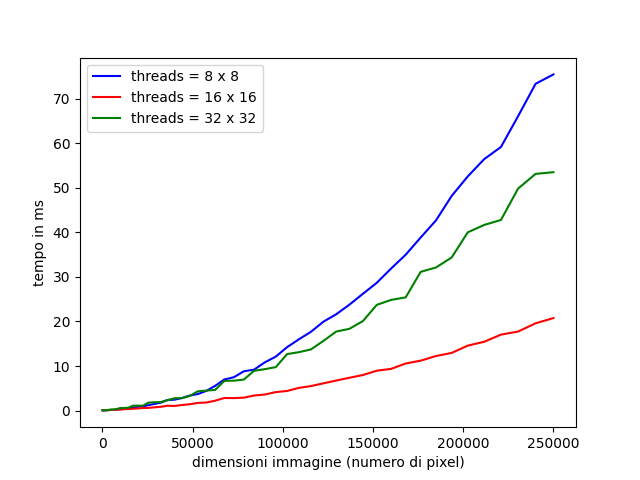
\includegraphics[width=0.9\linewidth]{test/gridTest/mul32/global_result.png} 
\caption{\small Tempo impiegato dall'esecuzione parallela (con memoria globale) al variare della dimensione dell'immagine.}
\label{t2_1}
\end{figure}
\begin{figure}[H]
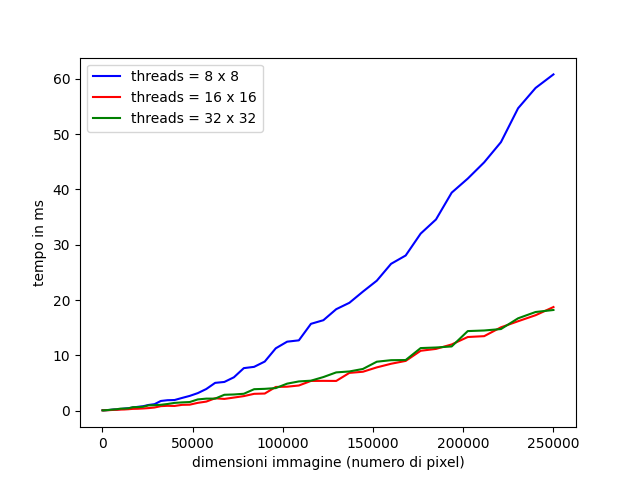
\includegraphics[width=0.9\linewidth]{test/gridTest/mul32/shared_result.png} 
\caption{\small Tempo impiegato dall'esecuzione parallela (con memoria shared) al variare della dimensione dell'immagine.}
\label{t2_2}
\end{figure}

Come si può osservare dai due grafici, in entrambi i casi la dimensione 8x8 si rivela essere la meno efficiente. Questo è dovuto al fatto che i block non sono occupati con una percentuale efficiente, comportando, quindi, una perdita di prestazioni dell'algoritmo.\\
\\
Per quanto riguarda la dimensione massima invece (32x32), questa comporta un miglioramento evidente nella versione shared, mentre continua a non essere così veloce per la versione con la global memory.\\
Questo miglioramento nella versione shared memory è dato dal fatto che la memoria allocata, essendo maggiore, permette meno accessi (non consecutivi) alla memoria globale e diminuisce il numero di fasi necessarie alla conclusione dell'algoritmo, portando a un miglioramento nei tempi.\\
\\
Infine, si può notare che la dimensione di mezzo (16x16) è la migliore per entrambi gli algoritmi.\\
Visto che tutti i thread nello stesso block eseguono le stesse azioni contemporaneamente, lo speedup ottenuto nella versione con global memory può essere spiegato dal fatto che il tempo impiegato per la gestione di 1024 thread da parte di un blocco è molto maggiore di quello impiegato per la gestione di soli 256 thread: il numero inferiore di block nel primo caso non porta ad una diminuzione del tempo di esecuzione abbastanza elevata da contrastare il tempo di gestione dei thread.\\
Per quanto riguarda la shared memory, invece, si può osservare che (nonostante la memoria allocata sia inferiore rispetto allo scorso caso), la velocità di esecuzione è simile a quella del caso precedente. La motivazione dietro a ciò riguarda, oltre alla gestione del numero dei thread da parte del block come per la global memory, anche il fatto che in questa versione dell'algoritmo siano presenti dei punti di sincronizzazione per tutti i thread di un block: in questo caso avere più block è vantaggioso, così mentre i thread di un block sono in attesa, quelli di un altro block possono continuare a operare sui dati.\\
\\
\\
Viste queste considerazioni, la dimensione dei block scelta per il test precedente (quello riguardante la variazione della dimensione dell'immagine) è stata la dimensione 16x16.\\


\subsection{Variazione del numero di thread - OpenMP}
Il secondo test svolto riguarda la modifica nel numero di thread nell'algoritmo parallelizzato tramite OpenMP.\\
Anche di questo test sono state fatte due versioni.

\subsubsection{Studio del livello di parallelizzazione}
Per capire quale dei tre possibili algoritmi OpenMP fosse il migliore, si è svolto un test in cui si osservano i tempi di esecuzione al variare del livello di parallelizzazione e del numero di thread utilizzati.\\
\\
Si sono lanciati cinque diversi algoritmi, con i seguenti parametri:
\begin{enumerate}
\item{primo livello - 15 thread;}
\item{secondo livello - 15 thread}
\item{entrambi i livelli - 15 thread nel primo livello, 1 nel secondo;}
\item{entrambi i livelli - 1 thread nel primo livello, 15 nel secondo;}
\item{entrambi i livelli - 15 thread nel primo livello, 15 nel secondo;}
\end{enumerate}
Ognuno di questi cinque algoritmi è stato fatto lavorare su immagini diverse per osservare come l'aumentare delle dimensioni (che vanno da 10x10 a 100x100 aumentando il lato di 5 in 5) influisse sui tempi di esecuzione.\\
Il grafico è in scala logaritmica lungo l'asse y\\
Di seguito il risultato:
\begin{figure}[H]
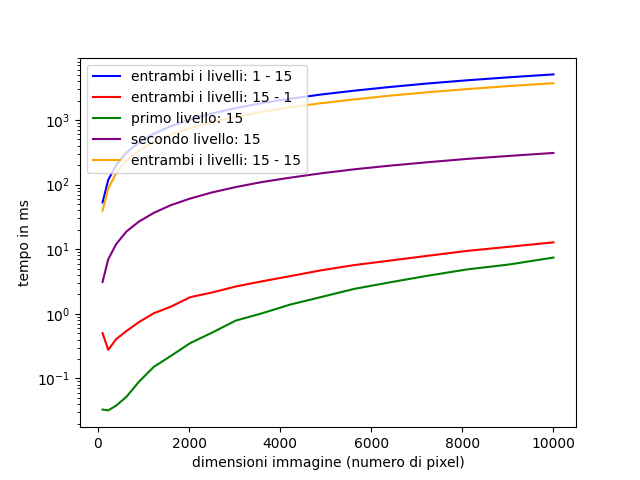
\includegraphics[width=1.1\linewidth]{test/threadsTest/levelsTest/result.png} 
\caption{\small Studio del livello di parallelizzazione degli algoritmi OpenMP}
\label{omp1}
\end{figure}
Osservando il grafico ottenuto, si possono fare le seguenti considerazioni:
\begin{enumerate}
\item{La parallelizzazione più efficiente è quella svolta al primo livello. Si noti che:
\begin{enumerate}
\item{la parallelizzazione al primo livello è migliore di quella al secondo livello perché la seconda viene invocata più volte (il tempo di gestione dei thread influisce maggioramente) e inoltre la seconda compie una reduction (più pesante del normale parallel for).}
\item{la parallelizzazione al primo livello è migliore di quella a entrambi i livelli perché la seconda comporta un'esplosione del numero di thread, andando in overhead e aumentando molto i tempi di esecuzione.}
\end{enumerate}}
\item{Mentre i tempi di esecuzione dell'algoritmo con parallelizzazione al primo livello e quello con una parallelizzazione a entrambi livelli con un solo thread nel secondo livello è simile (il fatto che il secondo algoritmo abbia un tempo di esecuzione leggermente maggiore è dato, ovviamente, dal dover gestire due diverse parallel region), lo stesso non si può dire per l'algoritmo con parallelizzazione al secondo livello e quello con parallelizzazione a entrambi livelli ma con un solo thread al primo livello. L'enorme differenza dei tempi (controintuitiva), in questo caso, può essere data da un'ottimizzazione diversa del compilatore per la generazione dei thread al secondo livello nei due diversi casi.}
\end{enumerate}

Da queste considerazioni, si deduce che il modo migliore per parallelizzare l'algoritmo con OpenMP è quello al primo livello.

\subsubsection{Studio del numero dei thread}
In questa seconda versione dell'esperimento si è osservato quale numero di thread potesse essere migliore per l'algoritmo di parallelizzazione al primo livello.\\
In particolare si sono lanciati tre versioni dell'algoritmo (uno con 10 thread, uno con 100 e uno con 1000) e si sono osservati i loro tempi di esecuzione al variare della dimensione dell'immagine (da 10x10 a 500x500, aumentando il lato di 10 in 10).\\
\\
Questi i risultati ottenuti:
\begin{figure}[H]
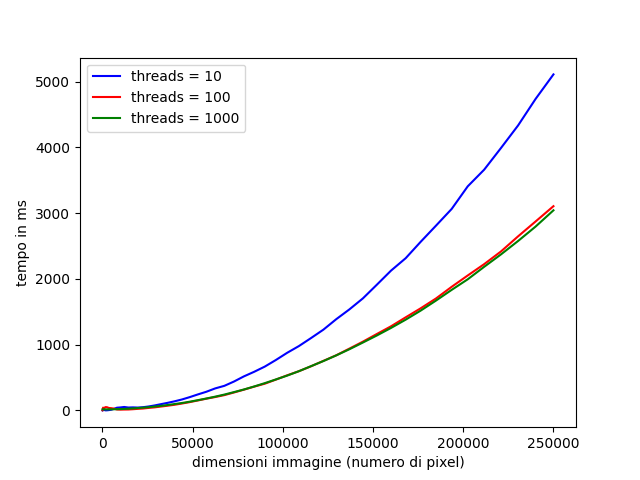
\includegraphics[width=1\linewidth]{test/threadsTest/velocityTest/result.png} 
\caption{\small Studio del numero dei thread}
\label{omp2}
\end{figure}

Come si può notare, l'aumento del numero di thread (anche molto elevato) non causa un rallentamento del programma, ma, mentre i tempi di esecuzione con 10 thread sono nettamente maggiori, la differenza dei tempi di esecuzione per gli altri due casi è quasi inesistente.\\
Questo è dato dal fatto che più è elevato il numero di thread, maggiore sarà anche il tempo di gestione di essi, e lo speedup ottenuto tenderà a annullarsi (e, con l'aumentare dei thread, a diventare negativo).\\
Vista la poca differenza dell'algoritmo tra l'utilizzo di 100 e 1000 thread, si è deciso di utilizzare il primo numero di thread nell'esperimento seguente.

\subsection{Variazione delle dimensioni dell'immagine}
Infine, in questo esperimento si è osservato lo speedup ottenuto dalla parallelizzazione su GPU (con shared memory) e da quella su CPU (al primo livello) a confronto con l’algoritmo sequenziale all’aumentare della dimensione dell’immagine.\\
\\
Il valore dei parametri di interesse è:
\begin{enumerate}[-]
\item{dimensioni dell'immagine che partono da 10x10 e arrivano fino a 500x500, aumentando il lato di 10 in 10 (quindi si sono svolte 50 iterazioni);}
\item{numero di thread per l'algoritmo in versione OpenMP = 100;}
\item{dimensioni dei block per CUDA = 16x16 (la grandezza della grid viene calcolata di conseguenza in base all'immagine), il miglior risultato dei test sulla dimensione dei block per CUDA.}
\end{enumerate}
Per questo grafico, vista l'enorme differenza tra i tempi di esecuzione, si è deciso di utilizzare una scala logaritmica lungo l'asse delle y.
\begin{figure}[H]
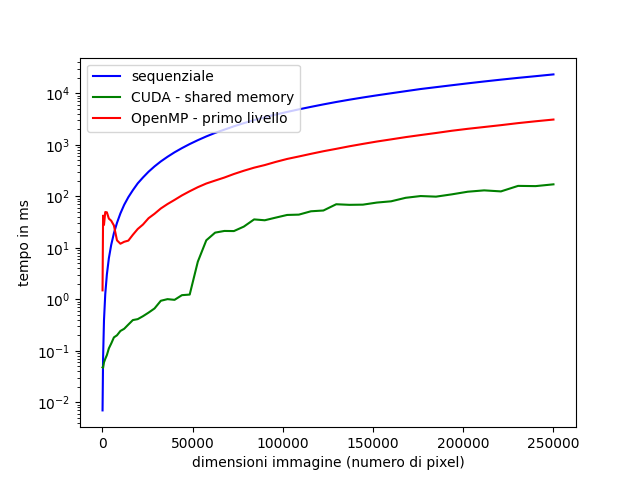
\includegraphics[width=1\linewidth]{test/dimTest/result.png} 
\caption{\small Tempo impiegato dall'esecuzione sequenziale e dalle due esecuzioni parallele al variare della grandezza dell'immagine.}
\label{tfinal}
\end{figure}
Attraverso questo esperimento si può dunque notare come la versione parallelizzata attraverso CUDA sia molto più veloce non solo della versione sequenziale ma anche della versione parallelizzata attraverso OpenMP. Questo prova come la parallelizzazione compiuta attraverso la GPU sia superiore di quella compiuta attraverso la CPU.\\
Inoltre la versione OpenMP scelta (con cioè 100 thread) è più lenta dell'algoritmo sequenziale per dimensioni dell'immagine molto piccole: ciò è ovviamente dato dal fatto che il tempo di gestione di ben 100 thread non viene bilanciato dall'esecuzione velocizzata su così pochi pixel.

\end{document}